\documentclass{article}
\usepackage{graphicx}
\usepackage{mathtools} % loads amsmath \usepackage{amsmath}
\usepackage{amssymb}
\usepackage{eqnarray}
\usepackage{bm}

\title{Notes MEP Tjip}
\author{chocolatetjipke }
\date{March 2026}

\def\dunder#1{\underline{\underline{#1}}}

\begin{document}

\maketitle

\section{proposal}
When generating hydrogen gas from renewable energy sources, it is one of the cleanest forms of energy. The exhausted gases from burning hydrogen are only water ($H_2O$). It is therefore very promising to look at energy solutions based around hydrogen. A difficulty of hydrogen gas is transport. Since the gas is so light, it isn't energy dense. Traditionally, we use high-pressure gas cylinders or liquefied hydrogen storage, which require either extremely high pressures (up to 700 bar) or very low temperatures (around $-253$C), creating safety risks and high energy costs. A new and improving way is to use metal hydride materials. These materials give high gravimetric and volumetric density, high $H_2$ absorption capacity, moderate working temperature, and moderate charging pressure for $H_2$ storage. A solution to the heat generation and requirement when charging and discharging these batteries is the use of phase change materials. The implementation of these materials gives us the freedom to not use heaters or coolers in these batteries. The goal of this thesis is to model and experiment with different battery setups using metal hydride materials together with these phase change materials.

We will be modelling this in Julia, a modern, high-performance programming language designed for technical and scientific computing. Julia offers a combination of ease of use, speed comparable to low-level languages, and strong support for functional and mathematical programming paradigms. We aim to apply finite element methods to model the adsorption of $H_2$ gas in the battery. Finite element methods provide flexibility in handling complex geometries and heterogeneous materials, allow precise spatial resolution of physical processes, and are well-suited for solving coupled multiphysics problems. When combined, we hopefully end with a powerful tool to explore different battery configurations, and to evaluate their efficiency and response time.

\section{Darzi}
\begin{itemize}
    \item Metal Hydride Tanks (MHTs)
    \item Phase Change Materials (PCMs)
\end{itemize}

We will be looking at Metal Hydride Tanks. `the formation of new bonds generates extra heat that must be removed to an external source. In turn the hydrogen desorption or discharge process requires breaking of bonds, compression of the crystal and hence the heat is sunk from the environment' together with `Thus, an effective passive heat transfer system could be a viable solution for cooling of MHTs during the charge process without the need for external energy [referring to internal cooling and heating systems]' leads to the implementation of PCMs: `Their results [Mellouli et al, 26 in Darzi] showed that the use of PCM could be a potential candidate for the metal hydride storage units'. Also important [Ben Maad, 27 and 28 in Darzi]: `Their result indicated that the metal hydrogen reactor can evacuate up to $80\%$ of the hydrogen stored by implementation of PCM without auxiliary heat sources'.

\subsection*{governing equations}

\begin{equation}
    (1-\epsilon )\frac{\partial \rho_s}{\partial t}=\dot m
\end{equation}

This is a coupling equation that couples the mass transfer of the whole volume ($\dot m$) to the mass transfer per unit volume of MHT tank. $\epsilon$ is the porosity, which can be seen as a measure for the amount of air (non-solid) in the volume, and thus the amount of solid (or MHT) is $(1-\epsilon)$.

\begin{equation}
    \epsilon \frac{\partial\rho_g}{\partial t}+\frac{1}{r}\frac{\partial}{\partial r}\left( r\rho_gu_r\right)+\frac{\partial}{\partial z}\left(\rho_g u_z\right) = \dot m
\end{equation}

Should come from conservation of mass:

\begin{equation}
    \frac{\partial \rho_g}{\partial t}+\nabla (\rho_g u_g) = -\dot m
\end{equation}

only weird thing is the swap in the sign of $\dot m$. I think it has to do with how you define it. In our case it is defined as change of mass going from `solid' to gas states. 

\subsection*{Absorption and desorption}

In Darzi Absorption and desorption are given by:
\begin{equation}\label{eq:adsorption_full_darzi}
    \dot m = C_a\left[\exp{\left(-\frac{E_a}{RT}\right)}\right]\left[ \ln\left( \frac{p_g}{p_{eq,a}}\right) \right]\left( \rho_{\text{sat}}-\rho_s\right)
\end{equation}

with $C_a$ absorption rate in $[s^{-1}]$. $p$ is pressure, and $p_{eq,a}$ is the equilibrium absorption pressure $[Pa]$. $E_a$ is the absorption activation energy in $[J/\text{mol}]$.

\begin{equation}
    \dot m =C_d
        \left[
            \exp{\left(-\frac{E_d}{RT}\right)}
        \right]
        \left[ 
            \ln\left( \frac{p_g-p_{eq,d}}{p_{eq,d}}\right) 
        \right]
        \left( \rho_{s}-\rho_\text{emp}\right)
\end{equation}

\subsection*{Momentum equations}
Now they go to the momentum equation(s)
\begin{align*}
    \rho_g\frac{\partial u_r}{\partial t} &= 
        -\frac{\partial p_g}{\partial r}
        -\rho_g\left( u_r\frac{\partial u_r}{\partial r} +u_z\frac{\partial u_r}{\partial z}\right)
        +\mu \left(
            \frac{\partial }{\partial r} \left( \frac{1}{r}\frac{\partial}{\partial r} (ru_r)\right)
            +\frac{\partial^2 u_r}{\partial z^2}
        \right) 
        - S_r\\
     \rho_g\frac{\partial u_z}{\partial t} &= 
        -\frac{\partial p_g}{\partial z}
        -\rho_g\left( u_r\frac{\partial u_z}{\partial r} +u_z\frac{\partial u_z}{\partial z}\right)
        +\mu \left(
            \frac{1}{r}\frac{\partial }{\partial r} \left( r\frac{\partial u_r}{\partial r} \right)
            +\frac{\partial^2 u_z}{\partial z^2}
        \right) 
        - S_z
\end{align*}
these have cartesian equivalences:
\begin{align*}
    \rho_g\frac{\partial u_x}{\partial t} &= 
        -\frac{\partial p_g}{\partial x}
        -\rho_g\left( u_x\frac{\partial u_x}{\partial x} +u_y\frac{\partial u_x}{\partial y}\right)
        +\mu \left(
            \frac{\partial^2 u_x}{\partial x^2}+\frac{\partial^2 u_x}{\partial y^2}
        \right) 
        - S_x\\
     \rho_g\frac{\partial u_y}{\partial t} &= 
        -\frac{\partial p_g}{\partial y}
        -\rho_g\left( u_x\frac{\partial u_y}{\partial x} +u_y\frac{\partial u_y}{\partial y}\right)
        +\mu \left(
            \frac{\partial^2 u_y}{\partial x^2}+\frac{\partial^2 u_y}{\partial y^2}
        \right) 
        - S_y\\
\end{align*}
or in vector notation:
\begin{equation}\label{eq:compressible_navier}
    \underbrace{\rho_g \partial_t \mathbf{u}}_{\text{Inertia}}=
    \underbrace{-\nabla p_g}_{\text{pressure force}} 
    -\underbrace{\rho_g (\mathbf{u}\cdot \nabla)\mathbf{u}}_{\text{advection}}+ 
    \underbrace{\mu \Delta \mathbf{u}}_{\text{viscous diffusion}}  - 
    \underbrace{\mathbf{S}}_{\text{viscous dissipation}}
\end{equation}
which together with conservation of mass gives all info about the movement of the gas
\begin{equation}\label{eq:conservation_off_mass}
    \frac{\partial \rho_g}{\partial t}+\nabla \cdot (\rho_g \mathbf{u}) = -\dot m
\end{equation}

\subsection*{energy/temperature}
system temperature is described as:

\begin{align*}
    (\rho C_{p} )_{\text{eff}}\frac{\partial T}{\partial t} + (\epsilon \rho_g C_{p,g}u_r \frac{\partial T}{\partial r}) + (\epsilon \rho_g C_{p,g}u_z \frac{\partial T}{\partial z})\\
    = \frac{1}{r}\frac{\partial}{\partial r}\left( rk_{\text{eff}}\frac{\partial T}{\partial r}\right)+\frac{\partial}{\partial z}\left( k_{\text{eff}}\frac{\partial T}{\partial z}\right)-\dot{m}((1-\epsilon)\Delta H+T(C_{p,g}-C_s))
\end{align*}

which again in simple $(x, y)$ coordinates becomes:
\begin{align*}
    (\rho C_{p} )_{\text{eff}}\frac{\partial T}{\partial t} + (\epsilon \rho_g C_{p,g}u_r \frac{\partial T}{\partial r}) + (\epsilon \rho_g C_{p,g}u_z \frac{\partial T}{\partial z})\\
    = \frac{1}{r}\frac{\partial}{\partial r}\left( rk_{\text{eff}}\frac{\partial T}{\partial r}\right)+\frac{\partial}{\partial z}\left( k_{\text{eff}}\frac{\partial T}{\partial z}\right)-\dot{m}((1-\epsilon)\Delta H+T(C_{p,g}-C_s))
\end{align*}

which in cartesian coordinate with $k_{\text{eff}}$ being constant becomes
\begin{equation}
    {(\rho C_{p} )}_{\text{eff}}\,\,{\partial_t T}
    = - \underbrace{\epsilon \rho_g C_{p,g} \mathbf{u}\cdot \nabla T}_{\text{convection}} 
    + \underbrace{k_{\text{eff}}\Delta T}_{\text{diffusion}}
    -\underbrace{\dot{m}((1-\epsilon)\Delta H+T(C_{p,g}-C_s)) }_{\text{heat due to mass trasfer}}
\end{equation}
with total unit of the equation: $\frac{J}{m^3s}$.

\subsection*{Summary}

Momentum:
\begin{equation}
    {\rho_g \partial_t \mathbf{v}}
    ={-\nabla p_g}
    -{\rho_g (\mathbf{v}\cdot \nabla)\mathbf{v}}
    +{\mu \Delta \mathbf{v}}
    -{\mathbf{S}}
\end{equation}
In $\left[\frac{kg}{m^2s^2}\right]$.\\
Mass:
\begin{equation}
    \begin{aligned}
        {\partial_t \rho_g}+\nabla \cdot (\rho_g \mathbf{v}) = -\dot m \\
        (1-\epsilon)\partial_t \rho_s = \dot{m}
    \end{aligned}
\end{equation}
In $\left[\frac{kg}{m^3s}\right]$.\\
Temperature/energy:
\begin{equation}
    {(\rho C_{p} )}_{\text{eff}}\,\,{\partial_t T}
    = - {\epsilon \rho_g C_{p,g} \mathbf{v}\cdot \nabla T}
    + {k_{\text{eff}}\Delta T}
    -{\dot{m}((1-\epsilon)\Delta H+T(C_{p,g}-C_s)) }
\end{equation}
with total unit of the equation: $\left[\frac{J}{m^3s}\right]$. \\
Equation of state:
\begin{equation}
    p_g = \rho_g RT    
\end{equation}
With absorption:
\begin{equation}
    \dot m = C_a\left[\exp{\left(-\frac{E_a}{RT}\right)}\right]\left[ \ln\left( \frac{p_g}{p_{eq,a}}\right) \right]\left( \rho_{\text{sat}}-\rho_s\right)
\end{equation}
and state vector:

\begin{equation}
    \mathbf{u} = \begin{pmatrix}
        \mathbf{v} \\ p \\ T \\ \rho_g \\ \rho_s
    \end{pmatrix}
\end{equation}
so it looks like it is 6 dimensional.
\subsection*{already solved}

\begin{equation}
\begin{aligned}
    \partial_t\rho_g&= D(\Delta\rho_g)-\mathbf{v}\cdot(\nabla\rho_g)-\dot m \\
    \partial_t\rho_s&=\dot m
\end{aligned}
\end{equation}
with
\begin{equation}
    \dot{m}      = a\rho_g(\rho_{\text{sat}}-\rho_s)
\end{equation}
and state vector:

\begin{equation}
    \mathbf{u} = \begin{pmatrix}
        \rho_g \\ \rho_s
    \end{pmatrix}
\end{equation}
and $\mathbf{v}$ given. I feel like my interpretation of rho is more of a `density of one fluid in a medium', than a general `this is the only material in this space so the total $kg/m^3$ is all there is here'.

\subsection*{Incompressible Navier Stokes}
The navier Stokes tutorial uses incompressible flow with the following governing equation and some crazy bc:
\begin{align}
    \partial_t v &= \nu \Delta v - (v\cdot \nabla) v -\nabla p \\
            0    &= \nabla \cdot v
\end{align}
their control vector therefor looks like
\begin{equation}
    \mathbf{u} = \begin{pmatrix}
        \mathbf{v} \\ p
    \end{pmatrix}
\end{equation}

\subsection*{simplification}
Darzi works with a (seemingly) 6-dimensional state vector. I think I can make some simplifications and reduce it to a $4$ dimensional vector. 

What I am now thinking of doing is a state vector:

\begin{equation}
    \mathbf{u} = \begin{pmatrix}
        \mathbf{v} \\ \rho_g \\ \rho_s
    \end{pmatrix}
\end{equation}

I lose the Temperature values in the state vector since I do not consider energy/temperature equations. If you do not do that $\rho_g$ and $p$ become linearly dependent on each other through the ideal gas law:

\begin{equation}
    p = \rho_g RT
\end{equation}

So removing temperature allows you to remove either pressure or density. I do not think we can calculate the charging of a battery with compressible navier stokes, so I want \underline{compressible} navier stokes:

\begin{equation}
    {\rho_g \partial_t \mathbf{v}}
    ={-\nabla p_g}
    -{\rho_g (\mathbf{v}\cdot \nabla)\mathbf{v}}
    +{\mu \Delta \mathbf{v}}
    -{\mathbf{S}}
\end{equation}

and conservation of mass equations:

\begin{equation}
    \begin{aligned}
        {\partial_t \rho_g}+\nabla \cdot (\rho_g \mathbf{v}) = -\dot m \\
        (1-\epsilon)\partial_t \rho_s = \dot{m}
    \end{aligned}
\end{equation}


\subsection*{Intermedeate Step}
I think the hardes upgrade is the loss of incompressibility, so I think I go look at those equations first. Maybe before adding mass transfer I look activation
\begin{equation}
    {\rho \partial_t \mathbf{v}}
    ={-RT\nabla \rho}
    -\mu \Delta \mathbf{v}
\end{equation}
with
\begin{equation}
        {\partial_t \rho} = -\nabla \cdot (\rho \mathbf{v})
\end{equation}
and state vector:
\begin{equation}
    \mathbf{u} = \begin{pmatrix}
        \mathbf{v} \\ \rho_g
    \end{pmatrix}
\end{equation}
above equations in 1D become:
\begin{equation}
    \begin{aligned}
        \rho \partial_t \mathbf{v}=-RT\partial_x \rho-\mu(\partial_x^2 v) \\
        \partial_t \rho = -\partial_x (\rho v)
    \end{aligned}
\end{equation}




\subsection*{Bluergh}
Newtons equation according to Wesseling:
\begin{equation}
U_t +f(U)_x=0, \quad U=\begin{pmatrix}\rho \\ m \\ \rho E \end{pmatrix}, \quad f = \begin{pmatrix}
m \\ m^2/\rho+p(\rho,r) \\ mH
\end{pmatrix}
\end{equation}

\newpage
\section{Stokes weak form/FEM}
Stokes takes into account both velocity $\mathbf{u}$ and pressure $p$ of the medium, where $u$ is a 2d vector where $u_1$ implies the velocity in the $x$-direction and $u_2$ in the $y$-direction. Stokes gives the following differential equations:

\begin{eqnarray}
    -\Delta \mathbf{u}+\nabla p &= b, \label{eq:stokes_momentum_strong} \\
    \nabla \cdot \mathbf{u} &= 0 \label{eq:stokes_pressure_strong},
\end{eqnarray}
Here, $b$ is the forcing term for momentum. 

For our weak form we will write $\mathbf{u}$ and $p$ as:

\begin{eqnarray}
    \mathbf{u} &= \sum_i^{N_u} \mathbf{u}^i \phi^i, \label{eq:stokes_expansion_momentum_u}\\
            p  &= \sum_i^{N_p}         p ^i \psi^i. \label{eq:stokes_expansion_pressure_p}
\end{eqnarray}
Where ${\phi}$ and $\psi$ are in \textbf{subspaces}. This gives us the solution vector:
\begin{equation}
    \mathbf{x} = \begin{pmatrix}
        u_x^1 \\ u_y^1 \\ u_x^2 \\ \vdots \\ p^{N_p-1} \\ p^{N_p}
    \end{pmatrix}
\end{equation}

Soon we will also work with test functions. For order sake I place the expansions of these below the expansions above:
\begin{eqnarray}
    \mathbf{v} &= \sum_i \mathbf{v}^i \phi^i, \label{eq:stokes_expansion_test_momentum_v}\\
            q  &= \sum_i         q ^i \psi^i. \label{eq:stokes_expansion_test_pressure_q}
\end{eqnarray}
Where the only difference is that these test functions live in the subspace \textbf{SUBSPACE}. Now we multiply Equations~\ref{eq:stokes_momentum_strong} with the test function $\mathbf{v}$, and integrate:

\begin{eqnarray*}
    \int_\Omega (-\Delta \mathbf{u}+\nabla p)\cdot\mathbf{v}dx &= \int_\Omega \mathbf{b}\cdot \mathbf{v}dx
\end{eqnarray*}

where we look at the first term of the integrant and see (I take a bit mroe time to write this example out, to show what happens and where the new notations come from. The rest will be done in quicker steps):

\begin{align*}
    \int_\Omega(-\Delta \mathbf{u})\cdot\mathbf{v} dx
    &=  \int_\Omega{ \begin{pmatrix}    
        \partial_x^2 u_1 + \partial_y^2 u_1\\
        \partial_x^2 u_2 + \partial_y^2 u_2
    \end{pmatrix}
        \cdot \begin{pmatrix}
            v_1 \\ v_2
        \end{pmatrix}dx} \\
    &= \int_\Omega (\partial_x^2 u_1)v_1+(\partial_y^2 u_1)v_1+(\partial_x^2 u_2)v_2+(\partial_y^2 u_2)v_2 dx \\
    &= \int_\Omega (\partial_x u_1)(\partial_x v_1) + (\partial_y u_1)(\partial_y v_1) \\ 
    &  \qquad +(\partial_x u_2)(\partial_x v_2) + (\partial_y u_2)(\partial_y v_2)dx\\
    &  \qquad - \int_{\delta \Omega} (\partial_x u_1 n_x+\partial_y u_1 n_y)v_1 + (\partial_x u_2 n_x+\partial_y u_2 n_y)v_2  dx \\
    &= \int_\Omega (\nabla \mathbf{u}):(\nabla \mathbf{v})dx - \int_{\delta\Omega}(\nabla \mathbf{un})\cdot \mathbf{v} dx
\end{align*}
Where the first term will be connected to the FEM, and the second term is from the boundary conditions. Here `:' is the Frobenius inner product defined as:

\begin{equation}\label{eq:Frobenius_inner_product}
    A:B :=\sum_{i,j}A_{ij}B_{ij},
\end{equation}

In Ferrite, we ignore the boundary term at first and make a `condition handler' object that will correct for it afterwards. Without the BC term we get the full expressions for the weak form of Equations~\ref{eq:stokes_momentum_strong}, and \ref{eq:stokes_pressure_strong} as:

\begin{align}
    \int_\Omega (\nabla\mathbf{u}):(\nabla\mathbf{v})-(\nabla \cdot \mathbf{v})p dx &= \int_{\Omega}\mathbf{b\cdot v}dx, \label{eq:stokes_momentum_weak}\\
    \int_\Omega q(\nabla\cdot\mathbf{u})&=0. \label{eq:stokes_pressure_weak}
\end{align}

Here $q$ is the test function for Equation~\ref{eq:stokes_pressure_strong}. What we now do (the Galerkin idea) is to create the matrix ($A$) that expands the finite element basis function of the above vector to the components that make the sum in the above Equations. The most complex part is again the first term of the integrant so we look at that first:

\begin{align}
    \int_\Omega (\nabla \mathbf{u}):(\nabla \mathbf{v})dx 
    &= \int_\Omega \sum_{i,j}(\nabla \mathbf{u})_{i,j}(\nabla \mathbf{v})_{i,j}dx\\
    &= \int_\Omega \sum_{i,j}(\partial_{x_j}u_i)(\partial_{x_j}v_i)dx \\
    &= \int_\Omega 
        \sum_{i,j}
            (\partial_{x_j}[\sum_k u_i^k\phi^k])
            (\partial_{x_j}[\sum_l v_i^l\phi^l])
        dx \\
    &= 
    \sum_{i,j,k,l}
        u_i^k v_i^l
        \int_\Omega 
            (\partial_{x_j}\phi^k)
            (\partial_{x_j}\phi^l)
        dx \label{eq:stokes_first_integrant}
\end{align}
Now if we want to calculate $A_{(i,m),(i,k)}^{uv}$ (which is to say the entry that corresponds with solution vector coefficient $u_i^k$, and test function $\phi^m\mathbf{e}_i$), we can substitute $\mathbf{v}=\phi^m\mathbf{e}_i$:
\begin{equation}
    A_{(i,m),(i,k)}^{uv} = \int_\Omega \nabla \phi^k\cdot\nabla\phi^m dx,
\end{equation}
all entries of the form $A_{(i,m),(j,k)}$ with $i\neq j$ are zero as seen in Equation~\ref{eq:stokes_first_integrant}. To get the coefficients of $A$ that correspond to $A_{(m),(i,k)}^{pv}$ (so the entries connecting solution vector coefficient $p^m$ and test function $\phi^m\mathbf{e}_i$), we do the same derivation as previous but with the second term in the integrant of Equation~\ref{eq:stokes_momentum_weak}. For the coefficients $A_{(i,m),(k)}^{uq}$ we look at Equation~\ref{eq:stokes_pressure_weak}. Doing both gives us:

\begin{align}
    A_{(m),(i,k)}^{pv} &= -\int_\Omega (\partial_{i} \phi^k)\psi^m dx \\
    A_{(i,m),(k)}^{uq} &= \int_\Omega  (\partial_{i} \phi^m)\psi^k dx
\end{align}
combining all (and realizing from the weak forms that there are no $A^{pq}$ terms), we get:

\begin{equation}
    A = \begin{pmatrix}
        A^{uv} & A^{pv} \\
        A^{uq} & \overline{0}
    \end{pmatrix}
\end{equation}
where $\overline{0}$ is the zero $N_p \times N_p$ matrix.
\newpage

\section{Navier Stokes}

\subsection*{incompressible flow}
First I wanted to look at incompressible flow. This is defined as:

\begin{equation}
    \frac{D \rho}{Dt} = 0
\end{equation}
which means there is no change in density following a fluid. This is defined as:

\begin{equation}\label{eq:navier_incompressibility_Drho}
    \frac{D\rho}{Dt}=\underbrace{\frac{\partial\rho}{\partial t}}_{\text{change at a fixed point}}+\underbrace{\mathbf{u}\cdot \nabla \rho}_\text{change due to movement}
\end{equation}
mass conservation then gives (no sources or sinks just yet):
\begin{align*}
    \frac{\partial \rho}{\partial t} &= -\nabla \cdot (\rho \mathbf{u}) \\
    &= -(\rho \nabla\cdot \mathbf{u}+\mathbf{u}\cdot \nabla\rho) \\
    \rightarrow \frac{\partial \rho}{\partial t}+\mathbf{u}\cdot \nabla\rho &=-\rho \nabla\cdot \mathbf{u} &\text{left-side Equation~\ref{eq:navier_incompressibility_Drho}}\\
    \rightarrow \nabla\cdot \mathbf{u} &= 0 \qquad &\text{if }\rho\neq 0
\end{align*}
which means we have divergence free flow. If we now look at the total volume of an incompressible medium in a tank we get:

\begin{equation}
    \frac{d}{dt}V_{\text{incompressible flow}}(t)=\int_{\Omega}\nabla \cdot \mathbf{u} dV = 0.
\end{equation}
This can also be expressed (divergence theorem), as the inflow of the tank:
\begin{equation}
    0 = \int_{\Omega}\nabla \cdot \mathbf{u} dV = \oint_{\delta\Omega}\mathbf{u\cdot n}\, dA
\end{equation}
so a tank with an incompressible medium inside has to have an inflow equal to the outflow!

\begin{figure}\centering
    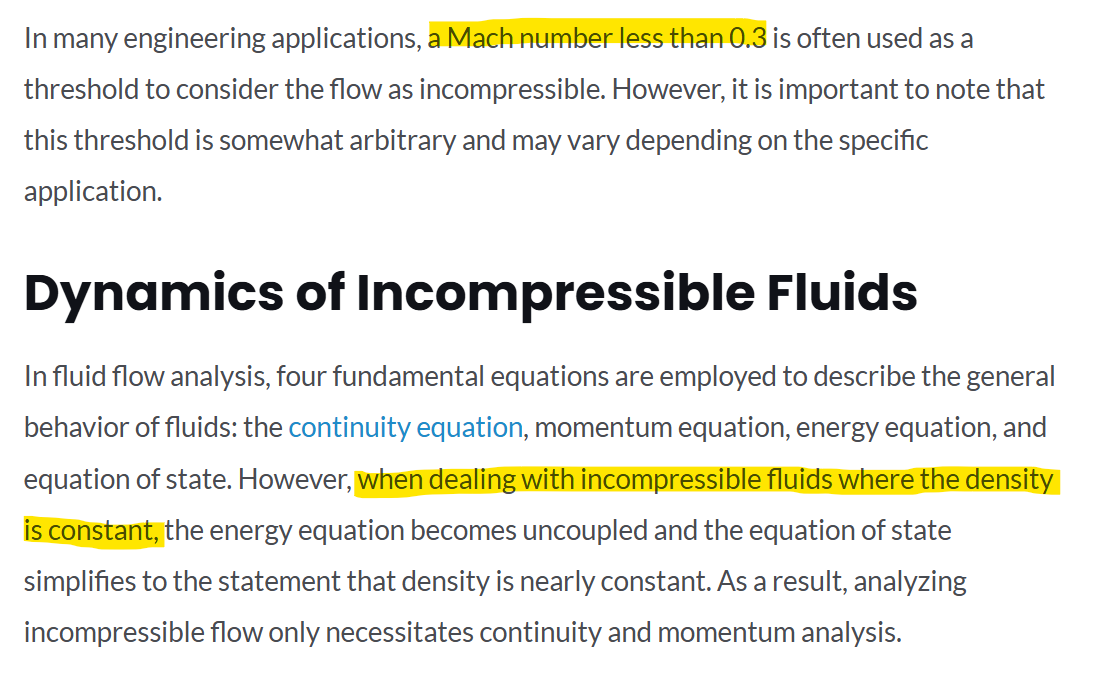
\includegraphics[width=.5\linewidth]{Figures/incompressible_liquid_gas.png}
    \caption{from https://engineerexcel.com/incompressible-fluid/}
\end{figure}

  
\subsection*{navier stokes}
From literature [SOURCE], we get Navier Stokes in the strong form as:

\begin{align}
    \partial_t \mathbf{u}&= \underbrace{\nu \Delta \mathbf{u}}_{\text{viscosity}} - \underbrace{(\mathbf{u}\cdot \nabla)\mathbf{u}}_{\text{advection}} - \underbrace{\nabla p}_{\text{pressure}} \label{eq:navier_velocity_strong}\\
    0 &= \underbrace{\nabla \cdot \mathbf{u}}_\text{incompressibility}
\end{align}

with $\mathbf{u}$ velocity field, $p$ the unknown pressure field, $\nu$ the dynamic viscosity and $\Delta$ the Laplacian. The weak form with $\mathbf{v}$, and $q$ give us a semi-discrete form (the derivative wrt time stays constant). The first and third terms of Equation~\ref{eq:navier_velocity_strong} are equivalent to their counterparts in Equation~\ref{eq:stokes_momentum_strong}. The second is left pretty much how it is and is our non-linear term. This gives us:

\begin{align}
\int_\Omega \partial_t \mathbf{u} \cdot \mathbf{v} \, dx
&=
\begin{aligned}[t]
  &- \int_{\Omega} \nu (\nabla \mathbf{u}) \colon (\nabla \mathbf{v}) \, dx \\
  &- \int_{\Omega} (\mathbf{u} \cdot \nabla)\mathbf{u} \cdot \mathbf{v} \, dx \\
  &+ \int_\Omega p (\nabla \cdot \mathbf{v}) \, dx \\
  &+ \int_{\partial \Omega} (\nu \partial_n \mathbf{v} - p \mathbf{n}) \cdot \mathbf{v} \, dx
\end{aligned} \label{eq:navier_momentum_weak}
\\
0 &= \int_\Omega (\nabla \cdot \mathbf{u}) q \, dx \label{eq:navier_pressure_weak}
\end{align}

\subsubsection*{Taylor Hood}
We need to find a higher order basis for the velocity term since it can become unstable otherwise. (pressure oscillations). (LOOK INTO THIS?)

\subsection*{stokes vs navier-stokes}
conceptual difference stokes/navier-stokes.
\textbf{stokes}:
\begin{equation}
    A\mathbf{x}=b
\end{equation}
\textbf{Navier}:
\begin{equation}
    M\mathbf{\dot{x}}=K\mathbf{x}+N(\mathbf{x})
\end{equation}

here we call $M$ the Mass matrix, $K$ the stiffness matrix, and $N$ represents the nonlinear advection term. Conceptually I want to look at this problem without a nonlinear term:

\subsubsection*{N=0}

without a non-linear term we get:
\begin{equation*}
    M\mathbf{\dot x}=K\mathbf{x}
\end{equation*}

here you can choose a finite difference sceme for time propagation (eg. backward Euler, Crank–Nicolson, Runge–Kutta). Say Backward Euler:

\begin{align*}
    \mathbf{\dot x}&\approx \frac{\mathbf{x}^{n+1}-\mathbf{x}^n}{\Delta t} \\
    \implies \qquad M\frac{\mathbf{x}^{n+1}-\mathbf{x}^n}{\Delta t}&= K\mathbf{x}^{n+1}\\
    \left( \frac{1}{\Delta t}M - K\right) \mathbf{x}^{n+1}&= \frac{1}{\Delta t}M\mathbf{x}^n
\end{align*}
(where the $=$-sign is dubious?) it is backwards Euler because we plug in $\mathbf{x}^{n+1}$ into the right side. We know $\mathbf{\dot x}^n$, so the right side is known and we can calculate as $b$ in the old Stokes examples.

\subsubsection*{Non linear terms}

Now what if $N$ is not zero. We again need to do an iterative method. Most commonly Newton-Rhapson. Given $x^n$ we get:

\begin{equation}
    F(\mathbf{x}^{n+1})=\frac{1}{\Delta t}M\mathbf{x}^{n+1} - K\mathbf{x}^{n+1}-N(\mathbf{x}^{n+1})-\frac{1}{\Delta t}M\mathbf{x}^n=0
\end{equation}
is what we want to solve. Do this in steps:
\vspace{.1in}

\textbf{Step 1}:

Initial guess: ${x^{(0)}=x^{n}}$

\vspace{.05in}

\textbf{Step 2}:

Calculate residual: $r = F(\mathbf{x}^{(k)})$

\vspace{.05in}

\textbf{Step 3:}:

Calculate Jacobian: $J = \frac {\partial F(\mathbf{x}^{(k)})}{\partial x}$

\vspace{.05in}

\textbf{Step 4}:

solve: $J(\mathbf{x}^{(k)}) = -F(\mathbf{x}^{(k)})$

\vspace{.05in}

\textbf{Step 5:}

Update $\mathbf{x}^{(k+1)}=\mathbf{x}^{(k)}+\mathbf{\partial x}^{(k)}$.

Repeat steps 2 - 5 until convergence.


\subsubsection*{non-linear N}

From Equation~\ref{eq:navier_momentum_weak}, the second term will be the starting point for our non-linear $\mathbf{N}(u)$.

\begin{align*}
    (\mathbf{u}\cdot \nabla)\mathbf{u}\cdot \mathbf{v} 
    &= \sum_l\sum_k\left( 
        \mathbf{u}^l\phi^l\cdot\nabla
    \right)
    (\mathbf{u}^k\phi^k) \cdot \mathbf{v}\\
    &= \sum_l\sum_k\left( 
        u_x^l\phi^l\partial_x+u_y^l\phi^l\partial_y
    \right)
    \begin{pmatrix}
        u^k_x\phi^k\\
        u^k_y\phi^k
    \end{pmatrix}
    \cdot \mathbf{v}\\
    &= \sum_l\sum_k 
    \begin{pmatrix}
        u_x^lu_x^k\phi^l(\partial_x\phi^k)+u_y^lu_x^k\phi^l(\partial_y\phi^k) \\
        u_x^lu_y^k\phi^l(\partial_x\phi^k)+u_y^lu_y^k\phi^l(\partial_y\phi^k) 
    \end{pmatrix}
    \cdot
    \mathbf{v} \\
    &= \sum_{i\in\{x,y\}}\sum_{j\in\{x,y\}}\sum_l\sum_k u_j^lu_i^k\phi^l(\partial_j\phi^k)v_i
\end{align*}
Once more to iterate the indeces: $i$ is the $x$ or $y$ index of $v_i$, $j$ is also a directional index but comes from the inner product $\mathbf{u}\cdot\nabla$. $l$ and $k$ iterate over the test functions of the two $\mathbf{u}$'s in our non-linear part of the equation. We introduce one more index: the index for corresponding to a test function if we set $\mathbf{v}=\phi^m\mathbf{e}_n$, where $m$ is the finite element basis function we want to construct $\mathbf{N}$ for, and $n$ is the dimension, again $n\in\{x,y\}$. This forces $i=n$, and gives us:

\begin{equation*}
    (\mathbf{u}\cdot \nabla)\mathbf{u}\cdot \mathbf{v} = \sum_{j\in\{x,y\}}\sum_l\sum_k u_j^lu_n^k\phi^l(\partial_j\phi^k)\phi^m
\end{equation*}
so now ${N_{(m,n)}}$, which is the part of $\mathbf{N}$ that corresponds with finite element test function $\phi^m\mathbf{e}_n$, becomes:
\begin{equation}\label{eq:Navier_non_linear_Nmn}
    N_{(m,n)}=\int (\mathbf{u}\cdot \nabla)\mathbf{u}\cdot \mathbf{v}_{(m,n)}dx = \sum_{j, l, k}\int u_j^lu_n^k\phi^l(\partial_j\phi^k)\phi^m dx
\end{equation}


\subsection*{Compressible Navier Stokes}
Compressible Navier Stokes is given as a starting point from Darzi as:

\begin{equation}
    \epsilon\frac{\partial\rho_g}{\partial t}+\nabla\cdot(\rho_g \mathbf{u})=\dot m
\end{equation}

Ideal gas law (also assumed by Darzi):
\begin{equation}
    \rho_g = \frac{P(t)M}{RT(t)},
\end{equation}

with $M$ molar mass of hydrogen, $P$ gas pressure, $R$ universal gas constant, and $T$ the temperature (want to make it time dependent in the future). These equations imply:

\begin{equation*}
    \implies \frac{\partial \rho_g}{\partial t}=\frac{M}{RT}\frac{\partial P}{\partial t}-\frac{PM}{RT^2}\frac{\partial T}{\partial t},
\end{equation*}

together with Darzy's law (explains movement of gases and fluids through porous media), equivalent to ohm-like laws:

\begin{equation}\label{eq:darcy}
    \mathbf{u}=-\frac{K}{\mu}\nabla P,
\end{equation}
here $K$ is the permeability, $\mu$ gas viscosity. This with the advection term in our Navier Stokes equation becomes:
\begin{equation}
    \nabla\cdot(\rho_g\mathbf{u}) = -\nabla\cdot(\rho_g\frac{K}{\mu}\nabla P)
\end{equation}
combining all previous equation gives our Navier Stokes as:

\begin{equation}
    \epsilon \frac{M}{RT}\frac{\partial P}{\partial t}-\epsilon\frac{PM}{RT^2}\frac{\partial T}{\partial t} +\nabla \cdot (\rho_g\frac{K}{\mu}\nabla P)=\dot m
\end{equation}

\section{first model}

Navier stokes initially gives:

\begin{equation}\label{eq:dummy_navier}
    \epsilon \partial_t \rho + \nabla \cdot (\rho \mathbf{u}) = \dot m
\end{equation}

If the gas comes in at a constant speed $v$ independent of place in a one dimensional tank, we get:
\begin{equation}\label{eq:dummy_navier_constant_u}
    \epsilon \partial_t \rho = - v\partial_x \rho
\end{equation}
with initial condition and boundary conditions:

\begin{equation*}
    \left\{ 
        \begin{aligned}
            p(x, 0) &= 0 \\
            p(0, t) &= 1            
        \end{aligned}
        \right.,
\end{equation*}
which we know how to solve. In general a one dimensional PDE as discussed is solved into:

\begin{equation*}
    \rho(x, t) = f(x-vt)
\end{equation*}
where the boundary condition and the initial condition imply:

\begin{equation*}
    f(z) = \left\{\begin{aligned}
        &1 \qquad z\leq 0 \\
        &0 \qquad z>0
    \end{aligned}\right.
\end{equation*}

\subsection*{dummy FEM}

if we want to solve this using a dummy finite element method, we start from Equation~\ref{eq:dummy_navier_constant_u}, and semi-discretize $\rho$ as:

\begin{equation*}
    \rho(x, t) = \sum_i \rho^i(t)\psi^i(x)
\end{equation*}

now we multiply by test function $q$ and integrating over $x$ gives:

\begin{align*}
    \int_\Omega (\partial_t\rho) (\partial_x p) dx &= -v \int \rho \partial_x
\end{align*}

\section*{contradiction in 1D battery}

Given a 1D battery of length L we get (from navier stokes):

\begin{align*}
    \partial_t v &= \nu \partial_{xx} v-v (\partial_x v)-\partial_x p\\
    0 &= \partial_x v
\end{align*}



\end{document}
